
\chapter[matplotlib]{Introduction to plotting with matplotlib / pylab}


\section[Overview]{A bird's eye view}

matplotlib is a library for making 2D plots of arrays in python.%
\footnote{This short guide is not meant as a complete guide or tutorial. There
  is a more comprehensive user's guide and tutorial on the matplotlib web-site
  at http://matplotlib.sf.net.%
} Although it has its origins in emulating the Matlab graphics commands, it
does not require matlab, and has a pure, object oriented API. Although
matplotlib is written primarily in python, it makes heavy use of NumPy and
other extension code to provide good performance even for large
arrays. matplotlib is designed with the philosophy that you should be able to
create simple plots with just a few commands, or just one!  If you want to see
a histogram of your data, you shouldn't need to instantiate objects, call
methods, set properties, and so on; it should just work.

The matplotlib code is divided into three parts: the \textit{pylab
interface} is the set of functions provided by the \texttt{pylab}
module which allow the user to create plots with code quite similar
to matlab figure generating code. The matplotlib frontend or \textit{matplotlib
API} is the set of classes that do the heavy lifting, creating and
managing figures, text, lines, plots and so on. This is an abstract
interface that knowns nothing about output formats. The \textit{backends}
are device dependent drawing devices, aka renderers, that transform
the frontend representation to hardcopy or a display device. Example
backends: PS creates postscript hardcopy, SVG creates scalar vector
graphics hardcopy, Agg creates PNG output using the high quality antigrain
library that ships with matplotlib, GTK embeds matplotlib in a GTK
application, GTKAgg uses the antigrain%
\footnote{http://antigrain.com%
} renderer to create a figure and embed it a GTK application, and so
on for WX, Tkinter, FLTK, \ldots{}.

For years, I used to use matlab exclusively for data analysis and
visualization. matlab excels at making nice looking plots easy. When
I began working with EEG data, I found that I needed to write applications
to interact with my data, and developed and EEG analysis application
in matlab. As the application grew in complexity, interacting with
databases, http servers, manipulating complex data structures, I began
to strain against the limitations of matlab as a programming language,
and decided to start over in python. python more than makes up for
all of matlab's deficiencies as a programming language, but I was
having difficulty finding a 2D plotting package -- for 3D VTK, which
is discussed at length below more than exceeds all of my needs.

When I went searching for a python plotting package, I had several
requirements: 

\begin{itemize}
\item Plots should look great - publication quality. One important requirement
for me is that the text looks good (antialiased, etc)
\item Postscript output for inclusion with \LaTeX{} documents and publication
quality printing
\item Embeddable in a graphical user interface for application development
\item The code should be mostly python so itis easy to understand and extend
-- users become developers!
\item Making plots should be easy -- just a few lines of code for simple
graphs
\end{itemize}
Finding no package that suited me just right, I did what any self-respecting
python programmer would do: rolled up my sleeves and dived in. Not
having any real experience with computer graphics, I decided to emulate
matlab's plotting capabilities because that is something matlab does
very well. This had the added advantage that many people have a lot
of matlab experience, and thus they can quickly get up to steam plotting
in python. From a developer's perspective, having a fixed user interface
(the pylab interface) has been very useful, because the guts of the
code base can be redesigned without affecting user code. 

Without further ado, let's create our first figure. This example uses
the matplotlib object oriented API. Most users use the pylab interface,
which will be discussed next and makes it easier to make plots because
a lot of the tedius work of creating and managing figures and figure
windows is done for you behind the hood. But since the real core of
the library is the object oriented API, I think it is a good place
to start. If you are developing a graphical user interface or making
plots on a web server, you probably want maximal control with no magic
going on behind the scenes -- this is where the matplotlib API should
be used. If you are just trying to make a figure for inclusion in
a paper or if your working interactively from the python shell, you'll
probably be happy with the pylab interface.

\lstinputlisting[caption={Creating a simple figure with the antigrain backend (generates PNG) using the object oriented matplotlib library}]{examples/mpl_agg_oo.py}

%
\begin{figure}
\begin{centering}
\includegraphics[width=4in]{fig/mpl_one_two_three}
\par\end{centering}

\caption{\label{fig:mpl_agg}A simple plot generated by the antigrain (Agg)
backend .}

\end{figure}



\section[pylab tutorial]{A short pylab tutorial}

Here is about the simplest code you can use to create a figure with
matplotlib using the pylab interface. In this section, I'm assuming
you are using ipython in the pylab mode -- see Section\ref{sec:ipython_pylab}
for details.

\begin{lyxcode}
peds-pc311:\textasciitilde{}>~pylab

Python~2.3.3~(\#2,~Apr~13~2004,~17:41:29)

Type~\char`\"{}copyright\char`\"{},~\char`\"{}credits\char`\"{}~or~\char`\"{}license\char`\"{}~for~more~information.

~

IPython~0.6.12\_cvs~-{}-~An~enhanced~Interactive~Python.

?~~~~~~~->~Introduction~to~IPython's~features.

\%magic~~->~Information~about~IPython's~'magic'~\%~functions.

help~~~~->~Python's~own~help~system.

object?~->~Details~about~'object'.~?object~also~works,~??~prints~more.

~

~~Welcome~to~pylab,~a~matplotlib-based~Python~environment

~~~~help(matplotlib)~->~generic~matplotlib~information

~~~~help(pylab)~~~~~~->~matlab-compatible~commands~from~matplotlib

~~~~help(plotting)~~~->~plotting~commands

~

In~{[}1]:~plot({[}1,2,3])

Out{[}1]:~{[}<matplotlib.lines.Line2D~instance~at~0xb557a86c>]
\end{lyxcode}
%
\begin{figure}
\begin{centering}
\includegraphics[width=5in]{fig/mpl_toolbar}
\par\end{centering}

\caption{\label{fig:mpl_toolbar}The matplotlib toolbar used to navigate around
your figure}

\end{figure}


If your settings are correct, a figure window should popup and you
should be able to interact with it. That's a lot less typing than
our initial example using the object oriented API in which you had
to manually create the Figure, Axes and so on!

Try clicking on the navigation toolbar at the bottom of the figure
-- the toolbar is shown in Figure\ref{fig:mpl_toolbar}. The first
three buttons from left to right in Figure\ref{fig:mpl_toolbar} are
\textit{home}, \textit{back} and \textit{forward}. These byttons are
are akin to the web browser buttons. They are used to navigate back
and forth between previously defined views. They have no meaning unless
you have already navigated somewhere else using the pan and zoom buttons
as described below. This is analogous to trying to click \texttt{Back}
on your web browser before visiting a new page --nothing happens.
The home button always takes you to the first, default view of your
data. 

The next to button moving right is the pan/zoom button, which looks
like a cross with arrows on the end (a \textit{fleur}). The pan/zoom
button button has two modes: pan and zoom (no surprise there, right?).
Click this toolbar button to activate this mode; you should see {}``pan/zoom
mode'' show up in the status bar. Then put your mouse somewhere over
an axes. To activate panning: press the left mouse button and hold
it, dragging it to a new position. If you press \texttt{x} or \texttt{y}
while panning, the motion will be contrained to the x or y axis, respectively
. To activate zooming, press the right mouse button, dragging it to
a new position. The x axis will be zoomed in proportionate to the
rightward movement and zoomed out proportionate to the leftward movement.
Ditto for the yaxis and up/down motions. The point under your mouse
when you begin the zoom remains stationary, allowing you to zoom to
an arbitrary point in the figure. You can use the modifier keys \texttt{x},
\texttt{y} or \texttt{CONTROL} to constrain the zoom to the x axes,
the y axes, or aspect ratio preserve, respectively.

The next button moving right is the \textit{zoom to rectangle button}
which has a magnifying glass over a piece of paper. The button is
striaghtforward and works in the standard way; when you click it,
you should see that it is activated by looking for {}``Zoom to rect
mode'' in the status bar, and then you select the rectangular region
you want to zoom in on.

The final button is the \textit{save button}, which will save your
figure in the current view. All of the {*}Agg backends know how to
save the following image types: PNG, PS, EPS, SVG. 

Let's make the same figure we made using the object oriented API above,
ie Figure\ref{fig:mpl_agg}, but this time using the pylab\lstinputlisting[caption={Creating a simple figure in pylab}]{examples/mpl_pylab.py}

As you can see there is basically a direct translation between the
OO interface and the pylab interface. When \texttt{plot} is called,
the pylab interface makes a call to the function \texttt{gca()} (``get
current axes'') to get a reference to the current axes. \texttt{gca}
in turn, makes a call to \texttt{gcf} ({}``get current figure'')
to get a reference to the current figure. \texttt{gcf}, finding that
no figure has been created, creates the default figure using \texttt{figure()}
and returns it. \texttt{gca} will then return the current axes of
that figure if it exists, or create the default axes \texttt{subplot(111)}
if it does not. The last line show is a GUI independent way of actually
creating a figure window, and is not required for image backends such
as postscript.

Thus a lot happens under the hood when you call plot, but for the
most part you don't need to think about it -- it just works. The important
thing to understand is that the pylab interface has a state, and keeps
track of the current figure and axes. All plotting commands target
the current axes, and you can manipulate which ones are current

\lstinputlisting[caption={Creating multiple subplots and plotting multiple lines in a single plot command}]{examples/mpl_subplot_demo.py}

%
\begin{figure}
\begin{centering}
\includegraphics[width=4in]{fig/mpl_subplot_demo}
\par\end{centering}

\caption{\label{fig:mpl_subplot}It's easy to create multiple axes and subplots.}

\end{figure}


In addition to creating multiple subplots, this example contains a
couple of new things. In the first plot command, the return value
is stored as \texttt{l1, l2} and the \texttt{set} command is used
to change a default line property. 

\begin{lyxcode}
l1,~l2~=~plot(t1,~f(t1),~'bo',~t2,~f(t2),~'k-{}-')

set(l1,~markerfacecolor='g')
\end{lyxcode}
\texttt{l1} and \texttt{l2} are \texttt{matplotlib.lines.Line2D} instances
and they are created by the \texttt{plot} command and added to the
current axes. This is the typical mode of operation of the axes plot
commands: they create a bunch of primitive objects (lines, polygons,
text, images), add them to the axes, and return them. In this example,
the line's \texttt{markerfacecolor} property is set with the \texttt{set}
command. In the next section, we'll look into matplotlibs \texttt{set}
and \texttt{get} introspection system and show how to use it to customize
your lines, polygons, text instances and images.


\section[set and get]{Set and get introspection}

Everything that goes into a matplotlib figure, including the \texttt{Figure}
itself, are all objects dervied from a single base class \texttt{Artist,}
and the pylab \texttt{set} and \texttt{get} commands provide a unified
way to configure them. Let's create a simple plot of random circles,
and use that to explore how \texttt{set} and get work. First the basic
plot -- we'll store the return value as lines. Note that \texttt{plot}
always returns a \textit{list} of lines; in the example above there
were two lines \texttt{l1} and \texttt{l2}, and in the example below
there is only a single element of the list lines. No matter: \texttt{set}
and \texttt{get} will work on a single instance or a sequence of instances

\lstinputlisting{snippets/mpl_plot_line.ipy}

%
\begin{figure}
\begin{centering}
\includegraphics[width=4in]{fig/mpl_set_get1}
\par\end{centering}

\caption{\label{fig:mpl_setget1}The default marker plot, before marker customization}

\end{figure}


The simple figure that was created, a scattering of blue circles at
random locations, is shown in Figure\ref{fig:mpl_setget1}. To see
a listing of the properties of the line, and what their current values
are, call \texttt{get(lines)} \lstinputlisting{snippets/mpl_get.ipy}
and to see the same listing of properties with information on legal
values you can set them to, call \texttt{set(lines)}\lstinputlisting{snippets/mpl_set.ipy}

OK, we have a lot of options here.  Let's change the marker properties,
and add a linesytle

\begin{lyxcode}
In~{[}20]:~set(lines,~markerfacecolor='green',~markeredgecolor='red',

~~~....:~~markersize=20,~markeredgewidth=3,~

~~~....:~linestyle='-{}-',~linewidth=3)


\end{lyxcode}
That's a lot of typing, but to great effect!  The same data set now
has quite a different appearance, which is shown in Figure\ref{fig:mpl_setget2}.
Note in the long listing output of the set(lines) command above the
markerfacecolor settable property is listed as

\begin{lyxcode}
markerfacecolor~or~mfc:~any~matplotlib~color~-~see~help(colors)
\end{lyxcode}
The \texttt{markerfacecolor} has an alias \texttt{mfc} to save typing,
and common colornames have abbreviations too, so the \texttt{set}
command above could just as well be written

\begin{lyxcode}
In~{[}20]:~set(lines,~mfc='g',~mec='r',~ms=20,~mew=3,~ls='-{}-',~lw=3)

%
\begin{figure}
\begin{centering}
\includegraphics[width=4in]{fig/mpl_set_get2}
\par\end{centering}

\caption{\label{fig:mpl_setget2}The default marker plot, before marker customization}

\end{figure}

\end{lyxcode}
Another nice thing about matplotlib properties is that you can pass
them in as keyword arguments to \texttt{plot} and they will have the
same effect, eg, you can create the identical plot with

\begin{lyxcode}


In~{[}6]:~plot(x,~y,~'o',~mfc='g',~mec='r',~ms=20,~mew=3,~ls='-{}-',~lw=3)

Out{[}6]:~{[}<matplotlib.lines.Line2D~instance~at~0xb40db42c>]


\end{lyxcode}
As noted above, \texttt{set} and \texttt{get} work on any \texttt{Artist},
so you can configure your axes or text instances this way.  Eg, \texttt{xlabel}
returns a \texttt{matplotlib.text.Text} instance \lstinputlisting{snippets/mpl_text_set.ipy}

\begin{lyxcode}

\end{lyxcode}
So you have a lot of possibilities to customize your text!  The most
common things people what to do are change the font size and color;
the results of this command on the xlabel are shown in Figure\ref{fig:mpl_setget2}.

\begin{lyxcode}


In~{[}25]:~set(t,~fontsize=20,~color='darkslategray')~
\end{lyxcode}


\section[matplotlibrc]{Customizing the default behavior with the rc file}

matplotlib is designed to work in a variety of settings: some people
use it in \char`\"{}batch mode\char`\"{} on a web server to create
images they never look at. Others use graphical user interfaces (GUIs)
to interact with their plots. Thus you must customize matplotlib to
work like you want it to with the customization file \texttt{.matplotlibrc},
in which you can set whether you want to just create images or use
a GUI (the backend setting), and whether you want to work interactively
from the shell (the interactive setting). Almost all of the matplotlib
settings and figure properties can be customized with this file, which
is installed with the rest of the matplotlib data (fonts, icons, etc)
into a directory determined by distutils. Before compiling matplotlib,
it resides in the same dir as \texttt{setup.py} and will be copied
into your install path. Typical locations for this file are 

\begin{lyxcode}
C:\textbackslash{}Python23\textbackslash{}share\textbackslash{}matplotlib\textbackslash{}.matplotlibrc~\textcolor{blue}{\#~windows}~/usr/share/matplotlib/.matplotlibrc~~\textcolor{blue}{\#~linux}
\end{lyxcode}

By default, the installer will overwrite the existing file in the install path,
so if you want to preserve yours, please move it to your \texttt{HOME} dir and
set the environment variable if necessary.  In the rc file, you can set your
backend, whether you'll be working interactively and default values for most of
the figure properties.

In the RC file, blank lines, or lines starting with a comment symbol,
are ignored, as are trailing comments. Other lines must have the format

\begin{lyxcode}
~key~:~val~\textcolor{blue}{\#~optional~comment}~
\end{lyxcode}
where \textit{key} is some property like \texttt{backend}, \texttt{lines.linewidth},
or \texttt{figure.figsize} and \textit{val} is the value of that property.
Example entries for these properties are

\begin{lyxcode}
\textcolor{blue}{\#~this~is~a~comment~and~is~ignored~}

backend~~~~~~~~~:~GTKAgg~~~~\textcolor{blue}{\#~the~default~backend~}

lines.linewidth~:~0.5~~~~~~~\textcolor{blue}{\#~line~width~in~points}~

figure.figsize~~:~8,~6~~~~~~\textcolor{blue}{\#~figure~size~in~inches~}
\end{lyxcode}
A complete sample rc file is included with the matplotlib distribution
and available online.%
\footnote{http://matplotlib.sourceforge.net/.matplotlibrc%
}


\section[Plot Types]{A quick tour of plot types}


\section{Images}

Matplotlib has support for plotting images with imshow and figimage.
In imshow, the image data is scaled to fit into the current axes,
and many different interpolation schemes are supported to do the resampling,
and in figimage, the image data are transferred as a raw pixel dump
to the figure canvas without resampling. You can add colorbars, set
the default colormaps, and change the interpolation schemes quite
easily. 

%
\begin{figure}
\begin{centering}
\includegraphics[width=4in]{fig/mpl_image_jet}
\par\end{centering}

\caption{\label{fig:mpl_imshow_jet}A simple image plot of a 2D matrix, using
nearest neighbor interpolation and the \texttt{jet} colormap.}

\end{figure}


\begin{lyxcode}
In~{[}15]:~x~=~arange(100.0);~x.shape~=~10,10

~

In~{[}16]:~im~=~imshow(x,~interpolation='nearest')

~

In~{[}17]:~colorbar()

Out{[}17]:~<matplotlib.axes.Axes~instance~at~0xb455496c>
\end{lyxcode}
which creates the image shown in Figure \ref{fig:mpl_imshow_jet}.
 You can interactively update the default colormap and change the
interpolation scheme, which creates the image show in Figure \ref{fig:mpl_imshow_hot}.

\begin{lyxcode}
In~{[}18]:~im.set\_interpolation('bilinear')

~

In~{[}19]:~hot()

%
\begin{figure}
\begin{centering}
\includegraphics[width=4in]{fig/mpl_image_hot}
\par\end{centering}

\caption{\label{fig:mpl_imshow_hot}The same image data, rendered with the
hot colormap and bilinear interpolation. matplotlib has 14 colormaps
built-in, and you can define your own with relative ease, and there
are 16 interpolation methods.}

\end{figure}

\end{lyxcode}
There is a lot more you can do with images: you can set the data extent
so that you can overlay contours or other plots, you can plot multiple
images to the same axes with different colors and transparency values,
you can load images with PIL or \texttt{imread} and plot them in matplotlib,
you can create montages of with \texttt{figimage} placed around the
figure window at different offsets, you can plot grayscale, rgb or
rgba data, and so on.  Consult the \textit{Matplotlib User's Guide}
and the \texttt{examples} subdirectory in the matplotlib source distribution
for more information. We'll clost off with a simple example of reading
in a PNG and displaying it

\begin{lyxcode}
In~{[}35]:~im~=~imread('../data/ratner.png')

~

In~{[}36]:~imshow(im)

Out{[}36]:~<matplotlib.image.AxesImage~instance~at~0xb3ffba2c>

~

In~{[}37]:~axis('off')

%
\begin{figure}
\begin{centering}
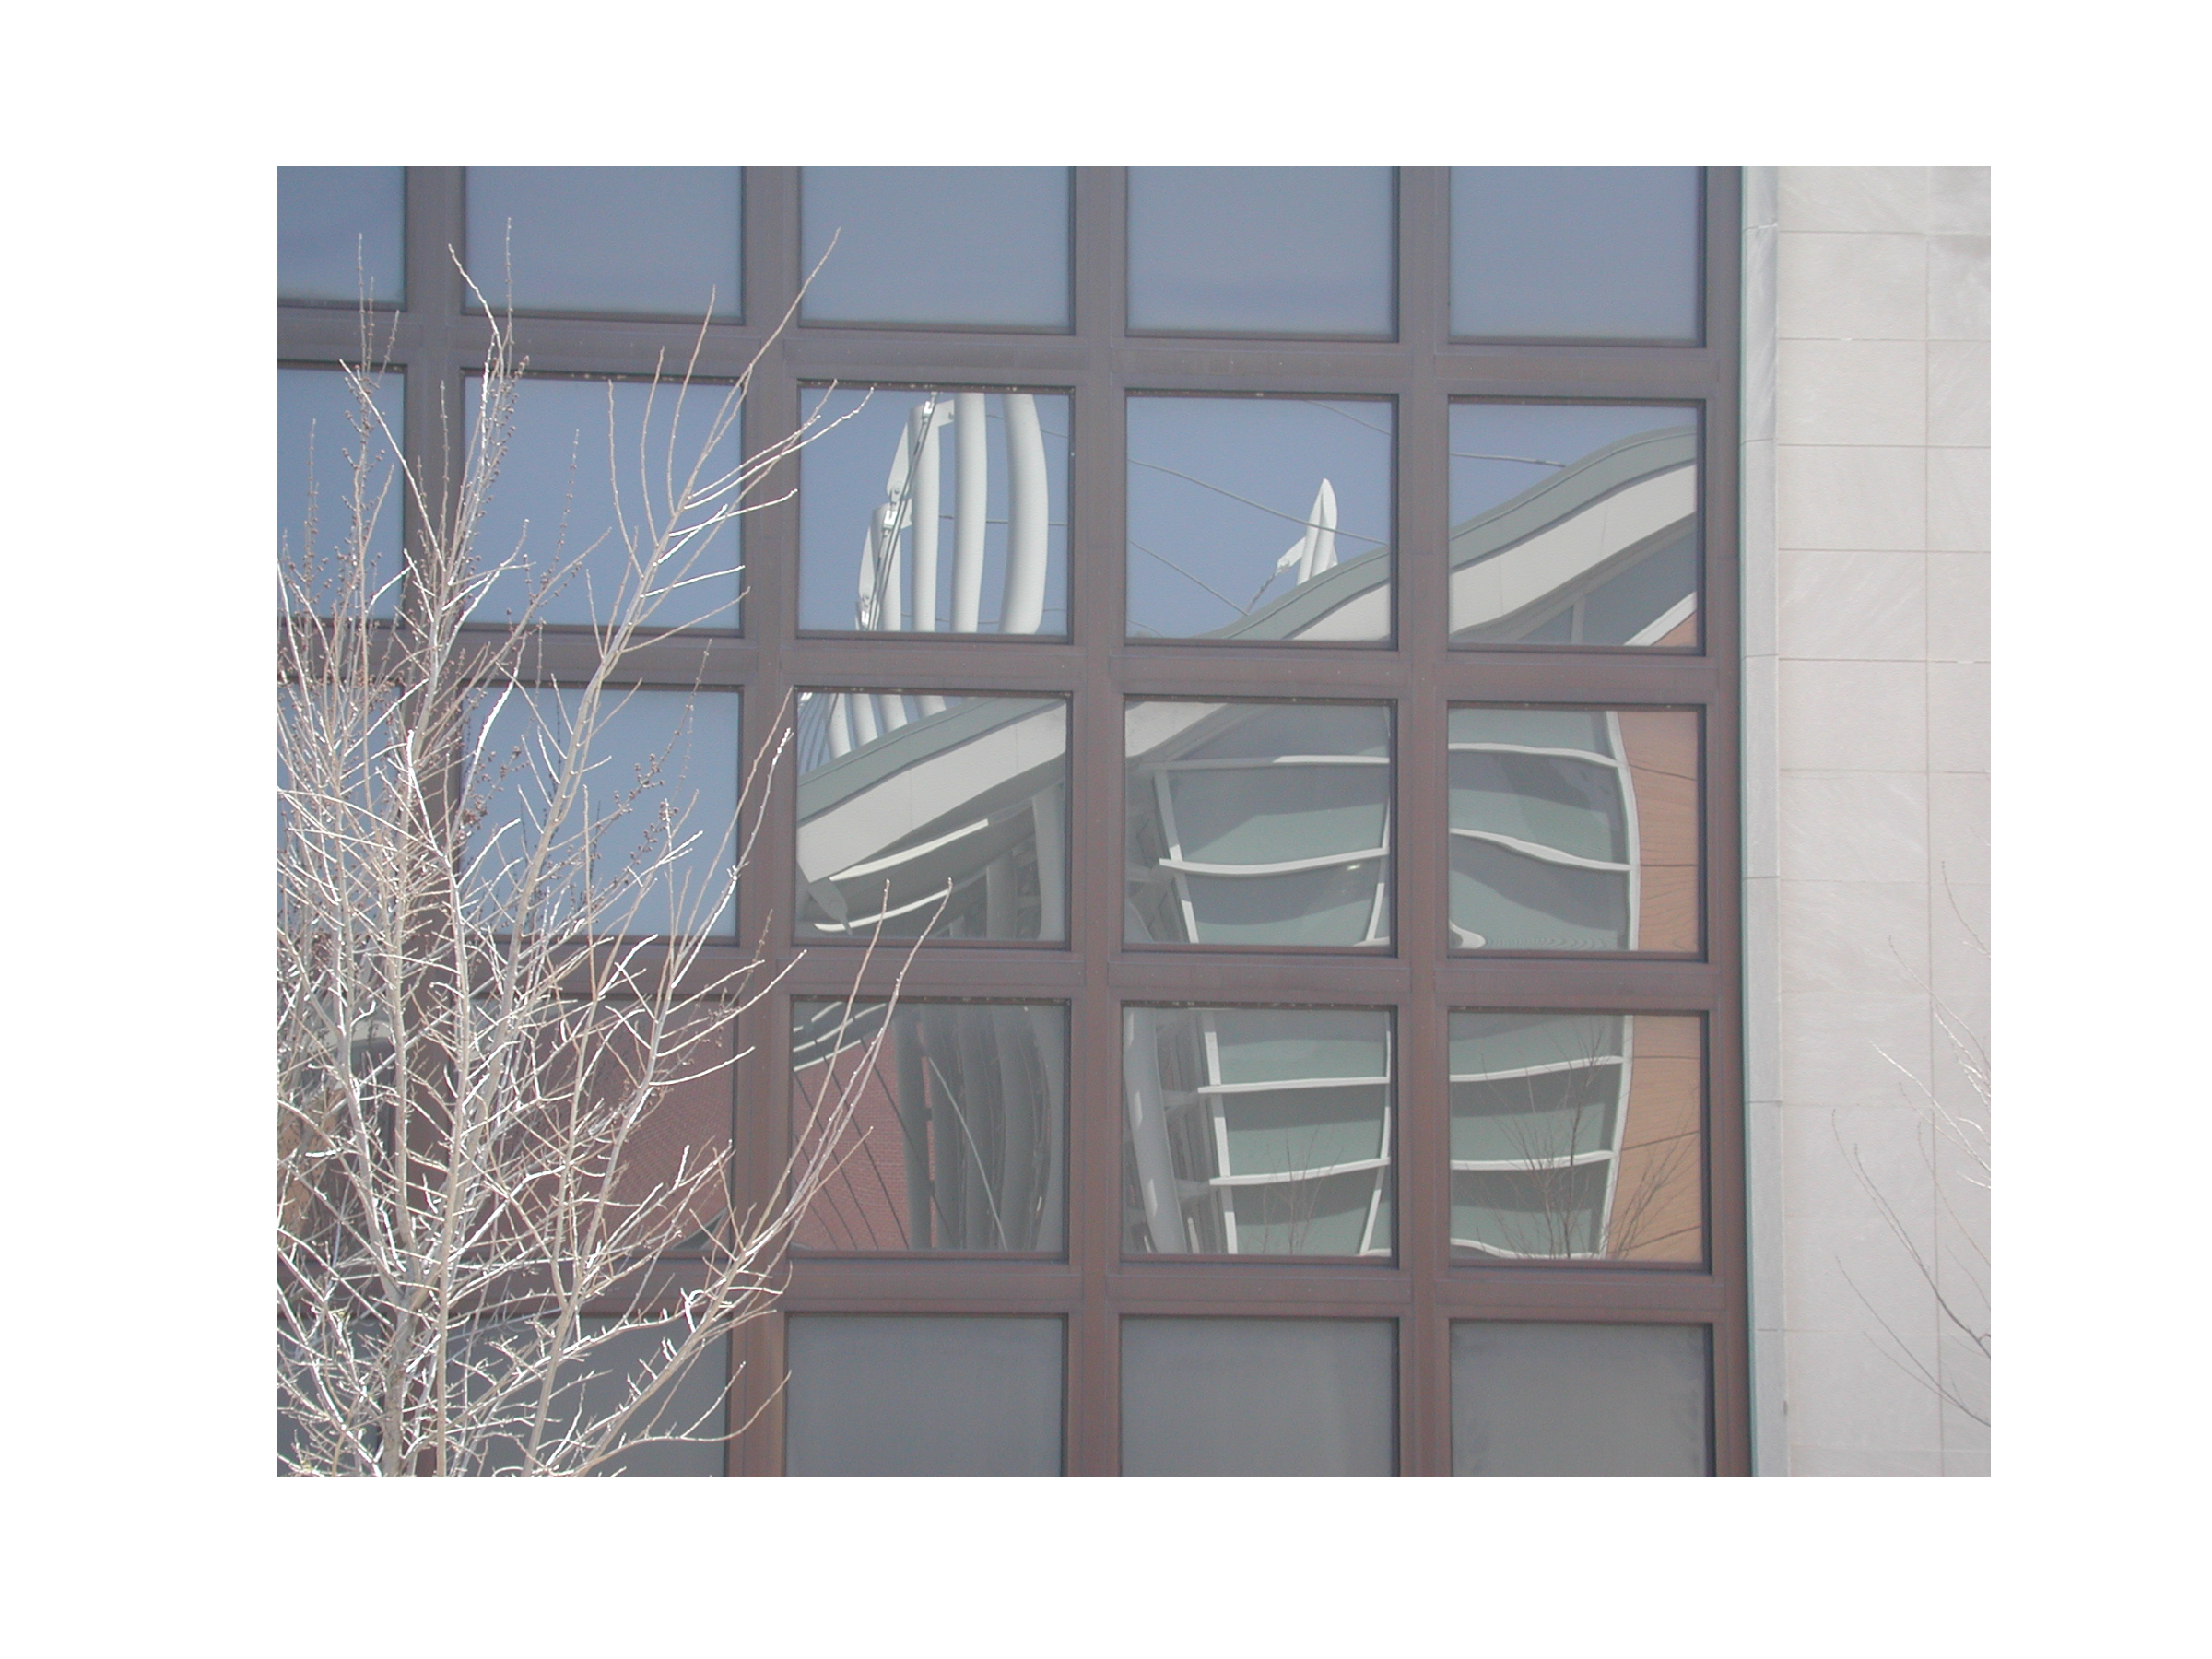
\includegraphics[width=5in]{fig/mpl_ratner}
\par\end{centering}

\caption{\label{fig:mpl_ratner}Displaying image data from your camera in matplotlib}

\end{figure}

\end{lyxcode}

\section[Text]{Customizing text and mathematical expressions}


\section[Event]{Event handling: Tracking the mouse and keyboard}
